\subsection{Key Expansion}
\label{sec:key-expansion}

The key expansion algorithm in \gls{AES} is responsible for generating the round keys (here on termed as subkeys) from the original cipher key. 
These subkeys are required at each round of the encryption and decryption processes. 
For an $N_r$-round \gls{AES} cipher, a total of $N_r + 1$ subkeys are needed (refer to Table~\ref{table:key-length-rounds}).

AES employs a word-oriented key schedule, where one word consists of 32 bits (4 bytes).
The generated subkeys are stored in a one-dimensional key expansion array $W$, which holds all the words produced during the expansion process.

In AES-128, the cipher key is 128 bits in length, which corresponds to 4 words. 
The key expansion produces 11 round keys, amounting to a total of 44 words ($W[0], \dots, W[43]$) (Figure \ref{fig:key-schedule-128}).
The initial key forms the first four words of the key expansion array:
\begin{equation}
    W[0], W[1], W[2], W[3] = \text{Original AES Key}
\end{equation}

For each subsequent group of 4 words, the first word is computed using a non-linear transformation function $g()$, and the remaining words are generated through a recursive \texttt{XOR} operation:
\begin{align}
    W[4i] &= W[4(i-1)] \oplus g(W[4i-1])\\
    W[4i+j] &= W[4i+j-i] \oplus W[4(i-1)+j]
\end{align}
where $i = 1,\dots,10$ corresponds to the round index and $j=1,2,3$ correspond to the subkey word index.

The function \texttt{g()} introduces non-linearity and diffusion into the key expansion process. 
It operates on a single 4-byte word and comprises three steps:
\begin{enumerate}
    \item \textbf{RotWord}: Performs a cyclic left shift on the input word by one byte.
    
    \textbf{Example:}
    \begin{align}
        \begin{pmatrix}
            B_0, B_1, B_2, B_3
        \end{pmatrix}
        \rightarrow
        \begin{pmatrix}
            B_1, B_2, B_3, B_0
        \end{pmatrix}
    \end{align}

    \item \textbf{SubWord}: Applies the \textsc{SubBytes} transformation to each byte of the word, substituting them using the AES S-Box (see Section \ref{sec:SubBytes}).
    
    \item \textbf{Round Constant (Rcon)}: Adds a round-dependent constant to the most significant byte of the word. 
    $\text{Rcon}[i]$ is defined as:
    \begin{equation}
        \text{Rcon}[i] = (r_i, 0, 0, 0)
    \end{equation}
    where $r_i = 2^{i-1}$ is computed in the finite field $GF(2^8)$
\end{enumerate}

The transformation \texttt{g()} plays a crucial role in strengthening the cipher by adding confusion and preventing linear relationships between the round keys and the original cipher key.

\begin{figure}[!ht]
    \centering
    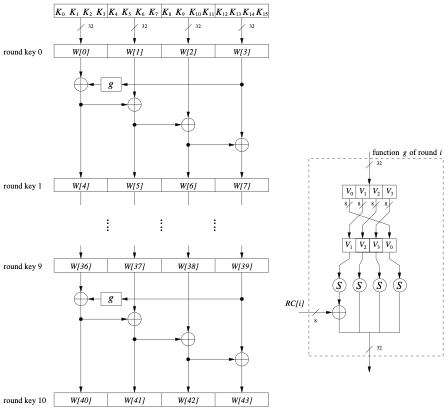
\includegraphics[width=\textwidth]{img/key-schedule-128.png}
    \caption{Key schedule for AES-128 \cite{Paar2024}.}
    \label{fig:key-schedule-128}
\end{figure}

AES-192 and AES-256 differ from AES-128 primarily in terms of their key length and the number of rounds executed during encryption.
For AES-192, the key expansion process generates 13 subkeys, totaling 52 words (Figure \ref{fig:key-schedule-192}). 
The computation of the key expansion array elements follows a procedure similar to AES-128; however, each iteration produces 6 new words instead of 4.
In the case of AES-256, 15 subkeys are generated, amounting to 60 words (Figure \ref{fig:key-schedule-256}). 
Each iteration of the key expansion calculates 8 words. 
Additionally, AES-256 employs an extra function, denoted as \texttt{h()}, which performs a \textsc{SubByte} transformation between the third and fourth words of each iteration, thereby increasing the complexity of the key schedule.

\begin{figure}[!ht]
    \centering
    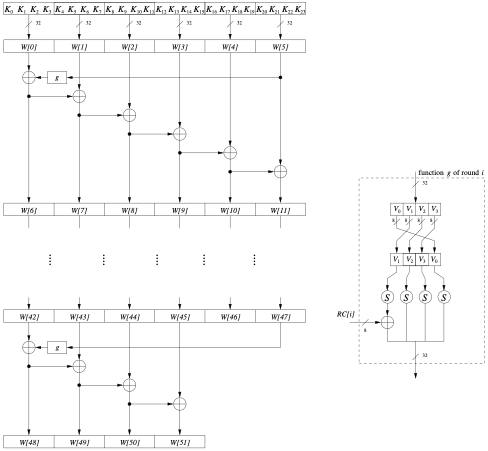
\includegraphics[width=\textwidth]{img/key-schedule-192.png}
    \caption{Key schedule for AES-192 \cite{Paar2024}.}
    \label{fig:key-schedule-192}
\end{figure}

\begin{figure}[!ht]
    \centering
    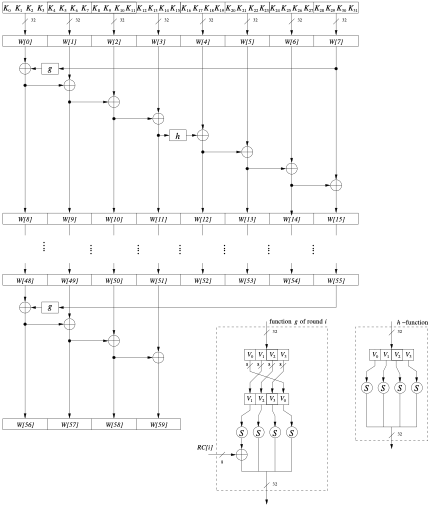
\includegraphics[width=\textwidth]{img/key-schedule-256.png}
    \caption{Key schedule for AES-256 \cite{Paar2024}.}
    \label{fig:key-schedule-256}
\end{figure}